\documentclass{standalone}
\usepackage[utf8x]{inputenc}
\usepackage{tikz}
% \usepackage{pgfplots,pgfplotstable}
\usepackage{color}

\usetikzlibrary{arrows,positioning} 
\definecolor{myorange}{RGB}{230,97,1}
\definecolor{mylightorange}{RGB}{253,184,99}
\definecolor{mypurple}{RGB}{94,60,153}
\definecolor{mylightpurple}{RGB}{178,171,210}
\definecolor{mycolor1}{RGB}{35,139,69}
\definecolor{mycolor2}{RGB}{102,194,164}
\definecolor{mycolor3}{RGB}{178,226,226}
\definecolor{mycolor4}{RGB}{237,248,251}

\begin{document}

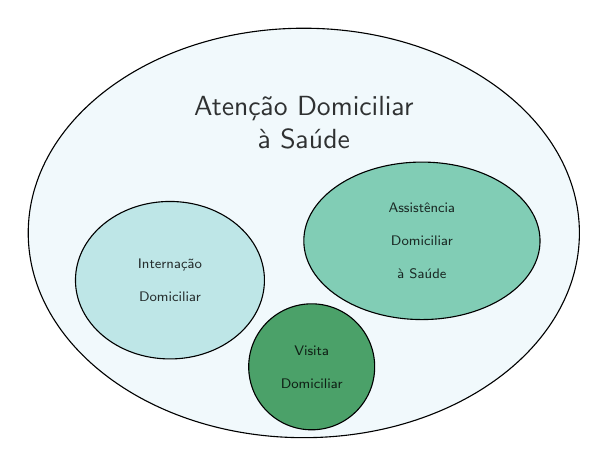
\begin{tikzpicture}[font=\sffamily]
  \begin{scope}[shift={(0cm,0cm)}, fill opacity=0.8]
    \draw[fill=mycolor4] (0,0) ellipse (3.5cm and 2.6cm); % atencao domiciliar
    \draw[fill=mycolor3] (-1.7,-0.6) ellipse (1.2cm and 1cm); % internacao domiciliar
    \draw[fill=mycolor2] (1.5,-0.1) ellipse (1.5cm and 1cm); % assistencia domiciliar
    \draw[fill=mycolor1] (0.1, -1.7) circle (0.8cm); % visita domiciliar

    \node at (0,1.4) [align=center]{Atenção Domiciliar\\ à Saúde};
    \node at (-1.7,-0.6) [align=center]{\tiny Internação\\ \tiny Domiciliar};
    \node at (1.5,-0.1)[align=center]{\tiny Assistência\\ \tiny Domiciliar\\ \tiny à Saúde};
    \node at (0.1,-1.7)[align=center]{\tiny Visita\\ \tiny Domiciliar};
  \end{scope}
\end{tikzpicture}

\end{document}
